\section{Introduction}
\label{section:introduction}

% {\color{blue} talk about the figures, try to highlight broader implications/operational problems. Main algorithmic insight is .... (1) our smoothing can be applied more broadly to other discrete event environments (2) our overall method of combining structure + data is useful. CLARIFY SAMPLE EFFICIENCY (learn more from a single trajectory)}

Queuing models are a powerful modeling tool to conduct performance analysis and optimize operational policies in diverse applications such as service systems (e.g., call centers~\cite{aksin2007modern}, healthcare delivery systems~\cite{armony2015patient}, ride-sharing platforms~\cite{banerjee2022pricing}, etc), computer and communication systems~\cite{harchol2013performance, neely2022stochastic}, manufacturing systems~\cite{shanthikumar2007queueing}, and financial systems (e.g., limit order books~\cite{cont2010stochastic}). Standard tools for queuing control analysis involve establishing structural properties of the underlying Markov decision process (MDP) or leveraging analytically more tractable approximations such as fluid~\cite{dai1995stability, chen1991discrete} or diffusion approximations~\cite{harrison1998heavy, stolyar2004maxweight, harrison1989scheduling, mandelbaum2004scheduling}. These analytical results often give rise to simple control policies that are easy to implement and interpret. However, these policies only work under restrictive modeling assumptions and can be highly sub-optimal outside of these settings. Moreover, deriving a good policy for a given queuing network model requires substantial queuing expertise and can be theoretically challenging. 

\begin{figure}[ht]
\hspace{-1em}
    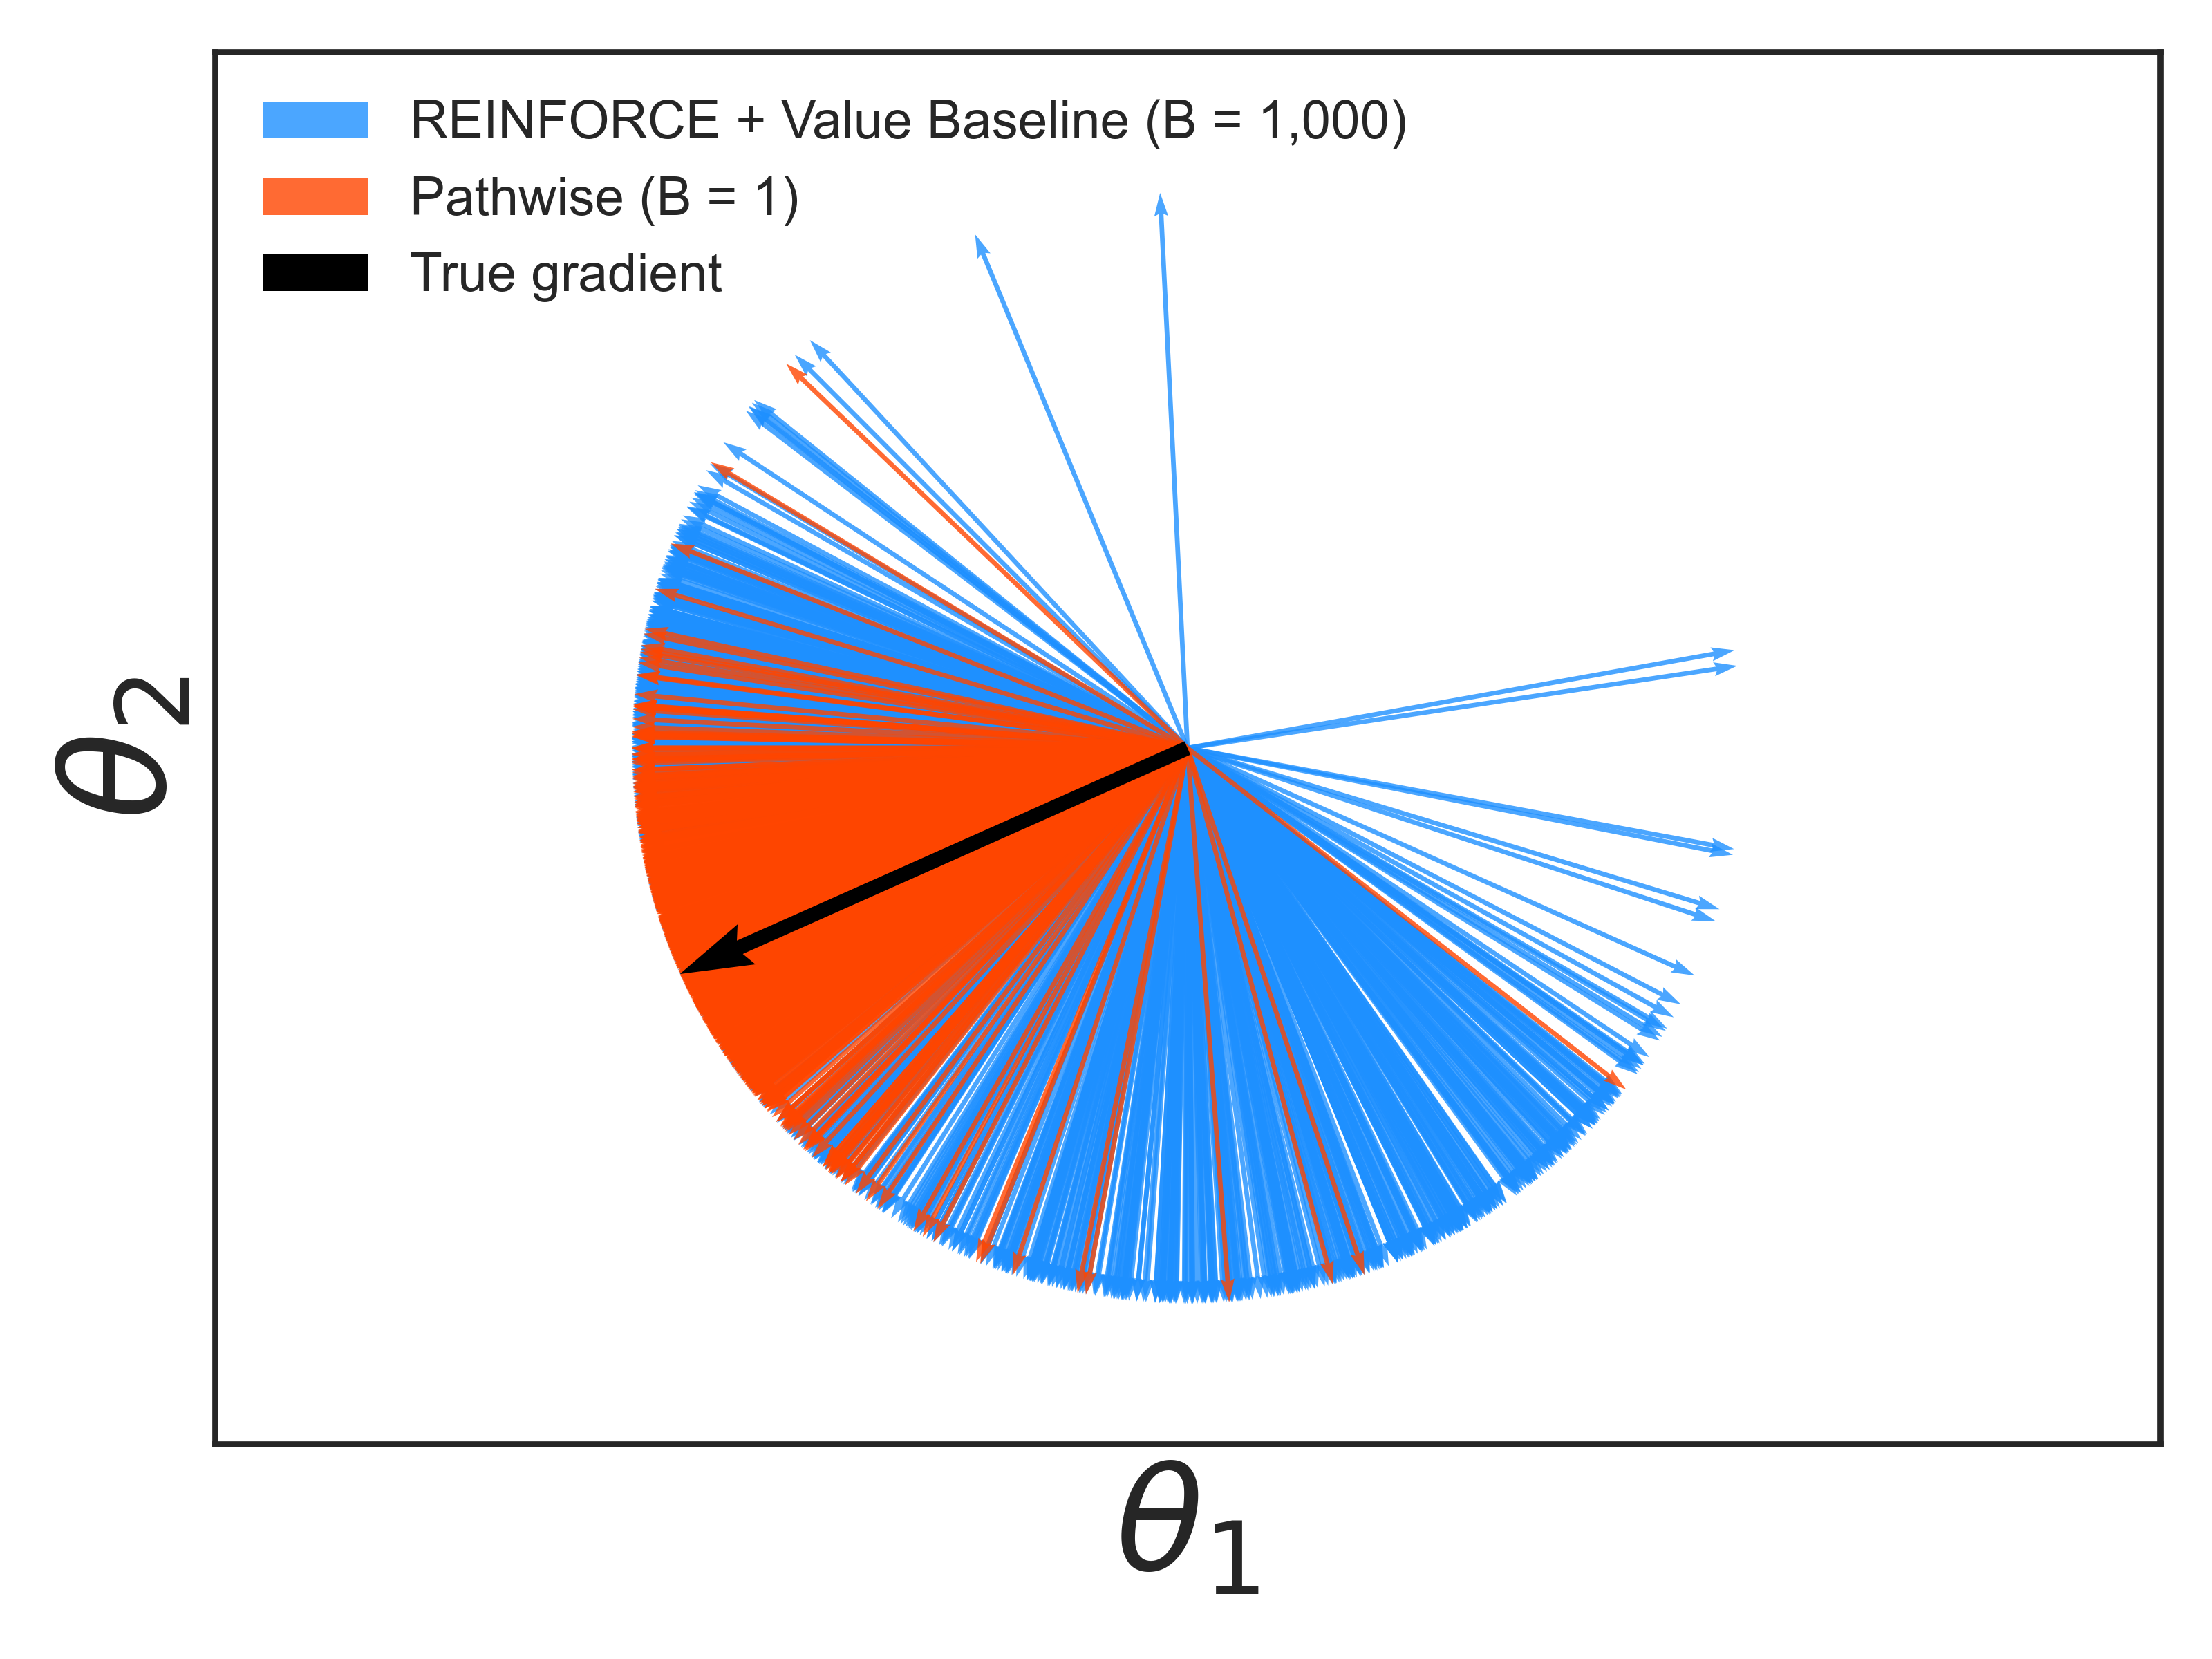
\includegraphics[height = 2.1in]{plot/gradient_eval/quiver_criss_cross_base_bh_0.9.png}
    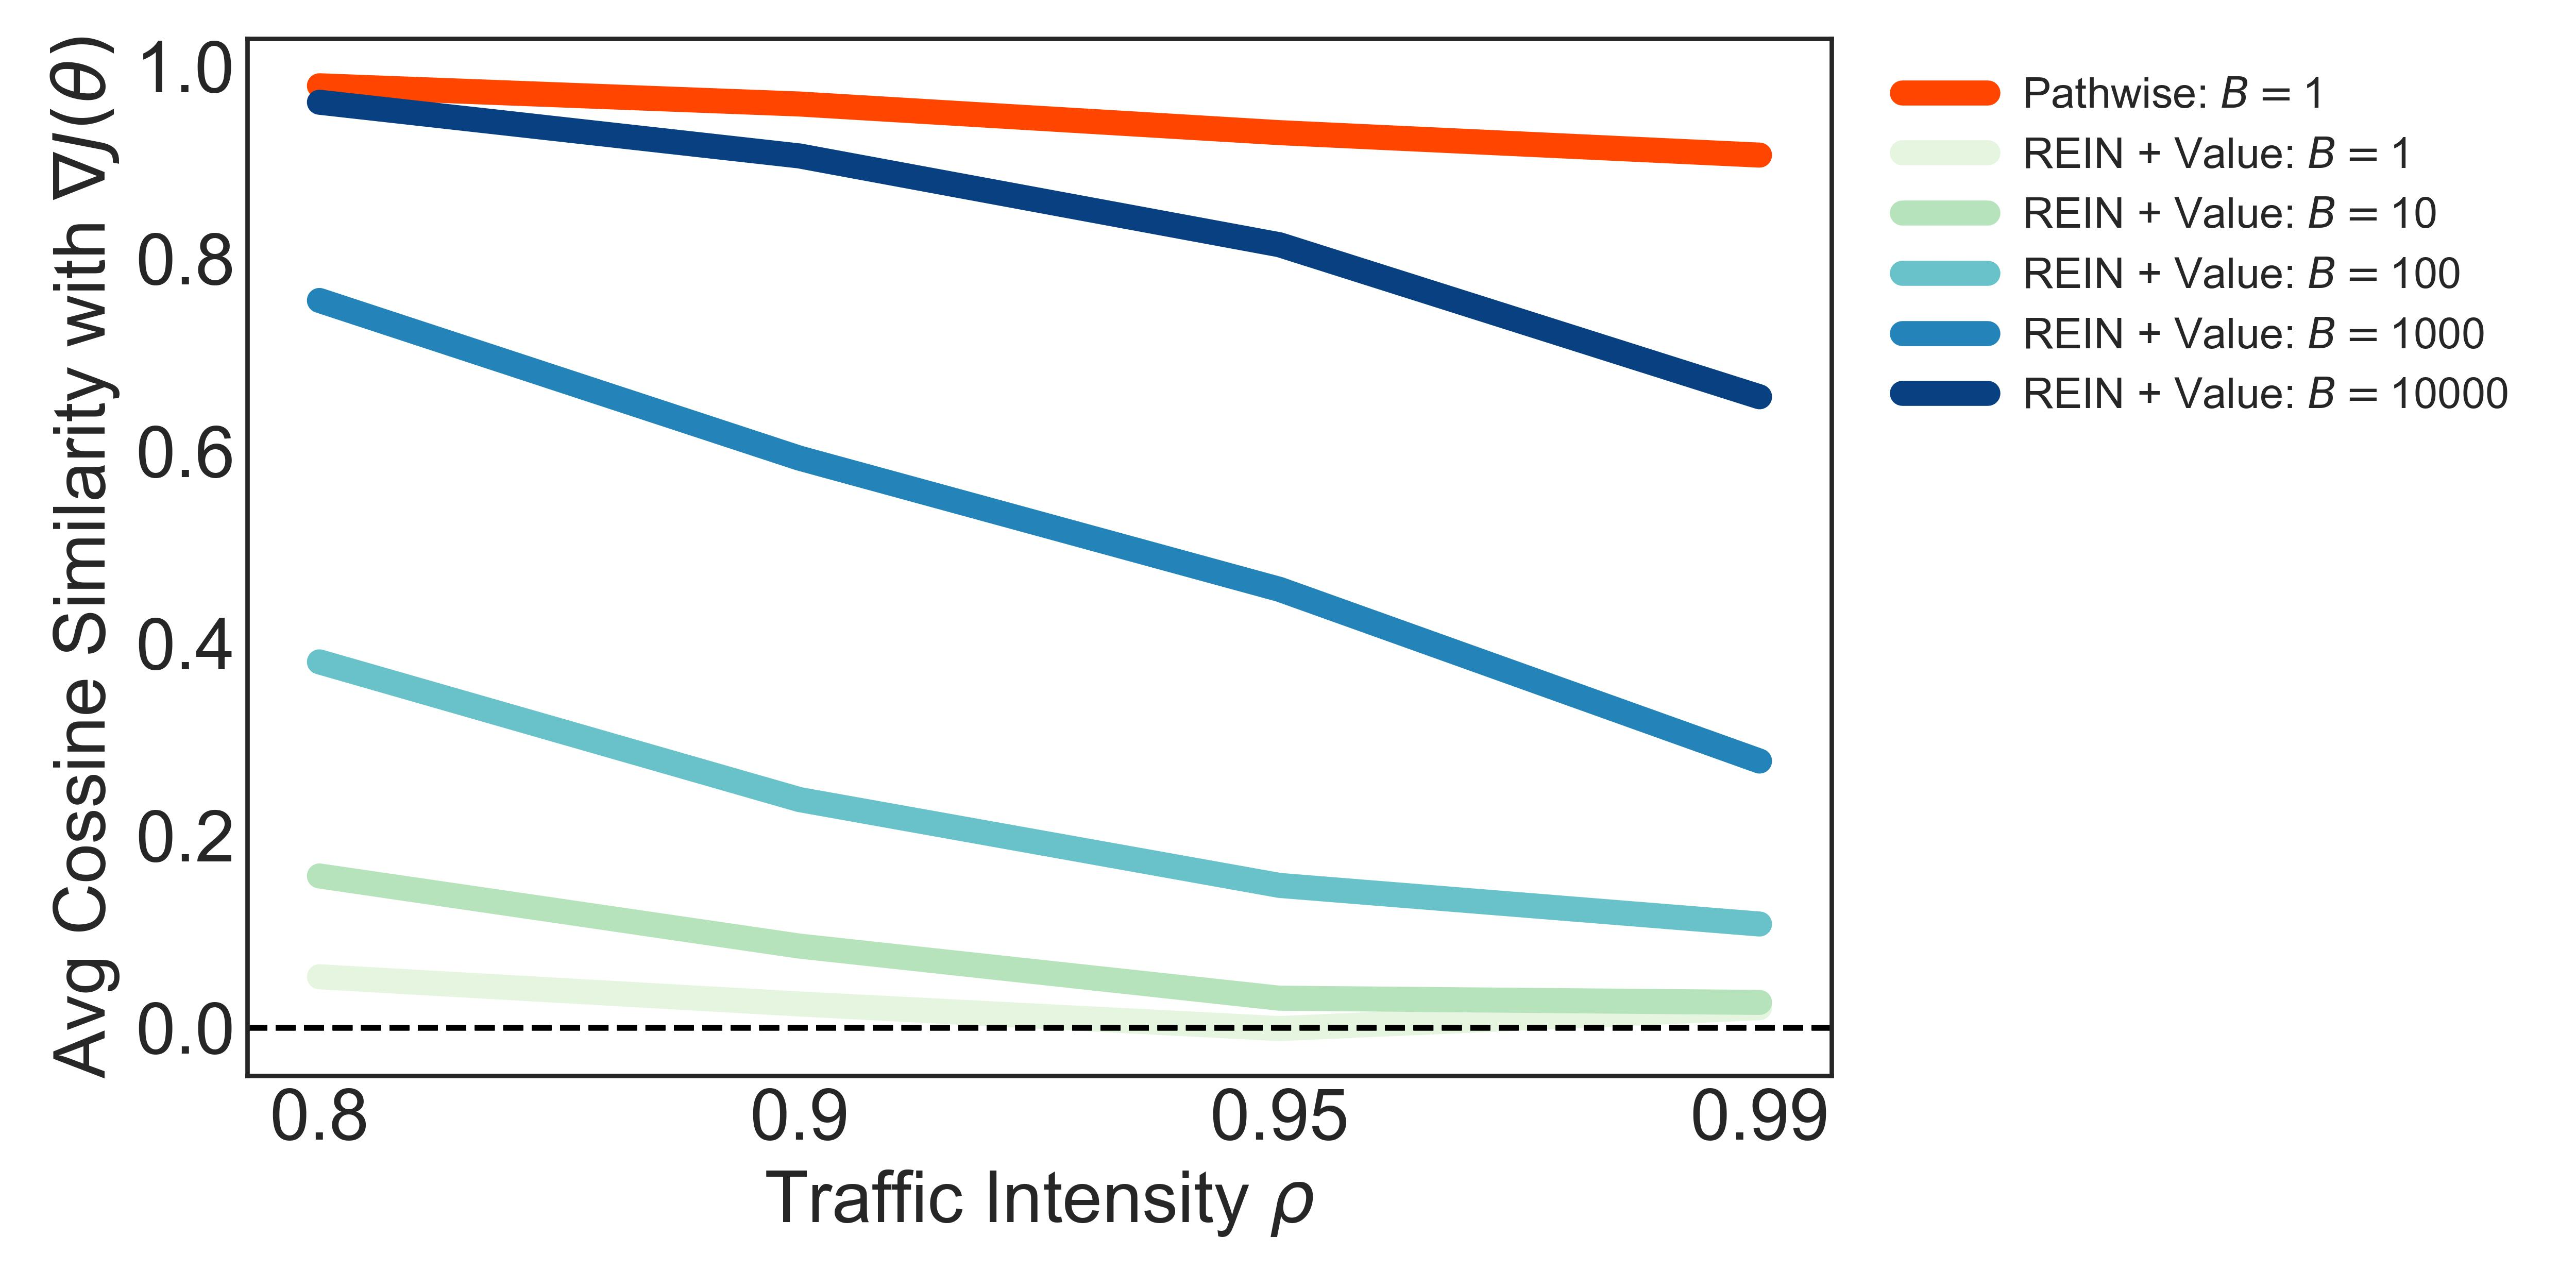
\includegraphics[height = 2.1in]{plot/gradient_eval/cossim_rho_baseline.jpg}
    
    \caption{Improvements in sample efficiency of our proposed $\pathwise$ policy gradient estimator over a standard model-free RL estimator, $\reinforce$. (Left) Samples of policy gradient estimators for a parameterized MaxPressure policy in a criss-cross network with traffic intensity $\rho=0.9$ (see Example~\ref{example:criss-cross}). Each draw of the $\reinforce$ estimator is averaged over $B = 10^3$ trajectories and is equipped with a value function baseline, which is fitted using $10^6$ state transitions. The $\pathwise$ estimator uses only a single trajectory, and no value function. Despite using less data, it is more closely aligned with the true gradient. (Right) Average cosine similarity (higher is better) of policy gradient estimators with the true policy gradient (see~\eqref{eqn:similarity} for more details) across different levels of traffic intensity for the criss-cross network. For $\reinforce$, we plot the cosine similarity of the estimator under different batch sizes $B=1,..,10^{4}$. We see that the efficiency advantages of $\pathwise$, with only 1 trajectory, are greater under higher traffic intensities, even outperforming $\reinforce$ with a value function baseline and $B=10^{4}$ trajectories.}
    \label{fig:gradient_cossim_eval} 
\end{figure}

Recent advances in reinforcement learning (RL) have spurred growing interest in applying learning methodologies to solve queuing control problems, which benefit from increased data and computational resources ~\cite{dai2022queueing,walton2021learning,liu2022rl}. These algorithms hold significant potential for generating effective controls for complex, industrial-scale networks encountered in real-world applications, which typically fall outside the scope of theoretical analysis. 
However, standard model-free RL algorithms~\cite{schulman2017proximal, schulman2015trust, mnih2016asynchronous} often under-perform in queuing control, even when compared to simple queuing policies~\cite{pavse2024learning, liu2022rl}, unless proper modifications are made. This under-performance is primarily due to the unique challenges posed by queuing networks, including (1) high stochasticity of the trajectories, (2) large state and action spaces, and (3) lack of stability guarantees under sub-optimal policies~\cite{dai2022queueing}.
For example, when applying policy gradient methods, typical policy gradient estimators based on coarse feedback from the environment (observed costs) suffer prohibitive error due to high variability (see, e.g., the $\reinforce$ estimators in Figure~\ref{fig:gradient_cossim_eval}). 

To tackle the challenges in applying off-the-shelf RL solutions for queuing control, we propose a new scalable framework for policy optimization that incorporates domain-specific queuing knowledge. Our main algorithmic insight is that queueing networks possess key structural properties that allow for several orders of magnitude more accurate gradient estimation. 
By leveraging the fact that the dynamics of discrete event simulations of queuing networks are governed by observed exogenous randomness (interarrival and service times), we propose a differentiable discrete event simulation framework. This framework enables the computation of a $\pathwise$ gradient of a performance objective (e.g., cumulative holding cost) with respect to actions. 

Our proposed gradient estimator, denoted as the $\pathwise$ estimator, can then be used to efficiently optimize the parameters of a control policy through stochastic gradient descent (SGD). By utilizing the known structure of queuing network dynamics, our approach provides finer-grained feedback on the sensitivity of the performance objective to any action taken along the sample path. This offers an infinitesimal counterfactual analysis: how the performance metric would change if the scheduling action were slightly perturbed.  
Rather than relying on analytic prowess to compute these gradients, we utilize the rapid advancements in scalable auto-differentiation libraries such as PyTorch~\citep{PaszkeGrChChYaDeLiDeAnLe17} to efficiently compute gradients over a single sample path or a batch of sample paths. 
Our proposed approach supports very general control policies, including neural network policies, which have the potential to improve with more data and computational resources. 
Notably, our method seamlessly handles large-scale queuing networks and large batches of data via GPU parallelization. Unlike off-the-shelf RL solutions whose performance is exceedingly sensitive to implementation details~\cite{huang2022implementation, ilyas2018closer}, our method is easy to implement (see e.g., Figure~\ref{fig:code}) and requires minimal effort for parameter tuning.

Across a range of queueing networks, we empirically observe that our $\pathwise$ estimator substantially improves the sample efficiency and stability of learning algorithms for queuing network control while preserving the flexibility of learning approaches.  In Figure~\ref{fig:gradient_cossim_eval}, we preview our main empirical findings which show that $\pathwise$ gradients lead to a 50-1000x improvement in sample efficiency over model-free policy gradient estimators (e.g., $\reinforce$~\cite{williams1992simple}). 
%in a variety of tasks and settings. 
Buoyed by the promising empirical results, we
provide several theoretical insights explaining the observed efficiency gains. 


\begin{figure}[t]
\centering
\hspace{-2em}
    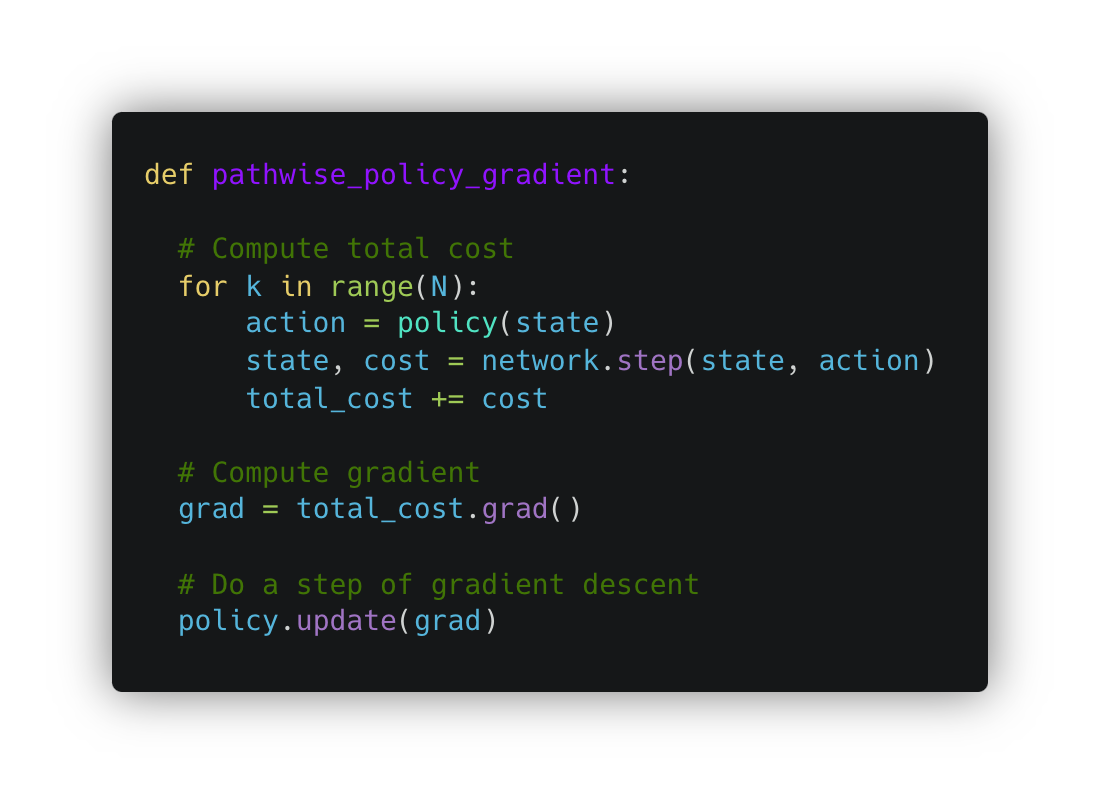
\includegraphics[height = 2.4in]{plot/gradient/pathwise_code.png}
    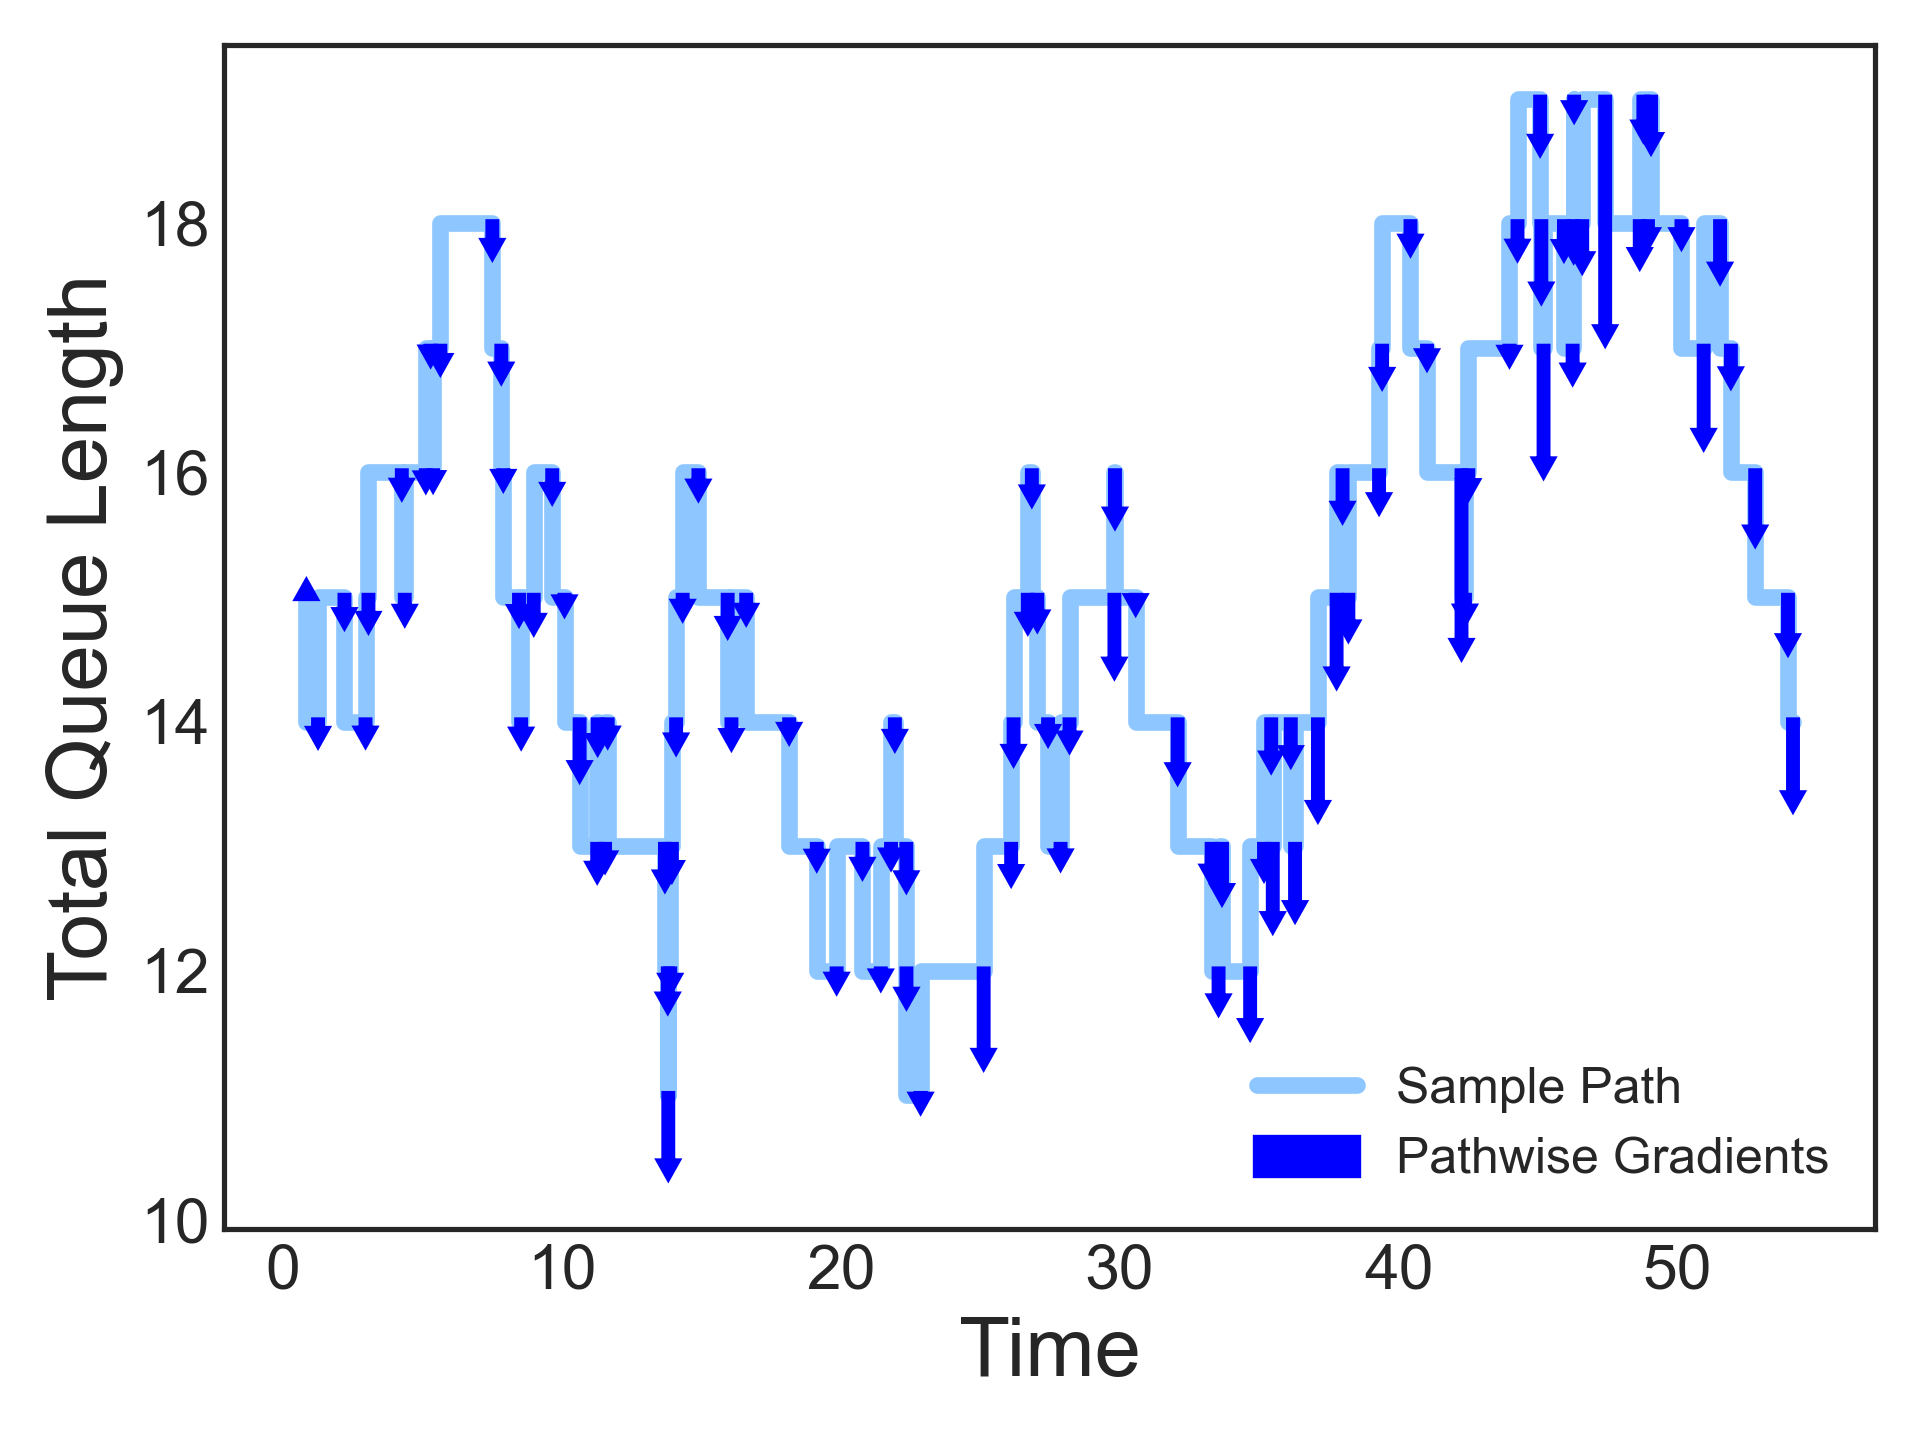
\includegraphics[height = 2.2in]{plot/sample_gradients.png}
    
\caption{(Left) Pseudo-code of a single gradient step of our proposed $\pathwise$ estimator. Computing the estimator requires only a few lines of code to compute the cost incurred by the policy. Once this cost is calculated, the sample path gradient is computed automatically via reverse-mode auto-differentiation. Unlike standard methods such as infinitesimal perturbation analysis or likelihood-ratio estimation, we can apply the same code for any network without any bespoke modifications. Unlike model-free gradient estimators like $\reinforce$, our method does not need a separate value function fitting step, managing a replay buffer, feature/return normalization, generalized advantage estimation, etc., as it has a low variance without any modification. (Right) A sample path of the total queue length (light blue) for a multi-class queuing network (see Example~\ref{example:multiclass}) under a randomized priority scheduling policy. Along the path, we display the gradients (dark blue) computed using our framework of the average cost with respect to each action produced by the policy: $\nabla_{u_{k}} \frac{1}{N}\sum_{k=0}^{N-1} c(x_{k},u_{k})\tau^{*}_{k+1}$.
    % (Right) Pseudo-code for a typical $\reinforce$ estimator is more involved, not only requiring the cost to be computed but also many additional steps, such as a value function fitting step to produce a baseline, management of a replay buffer, and normalization of states, costs, and returns which must be carefully tuned~\cite{engstrom2020implementation}. For modern policy gradient algorithms such as PPO~\cite{schulman2017proximal}, additional features are required, such as clipping of the advantages, monitoring the KL-divergence between iterates, etc. As a result, standard implementations often involve more than 10,000 lines of code, spread across multiple modules~\cite{huang2022cleanrl}.
    }
    \label{fig:code}
\end{figure}

Our proposed approach draws inspiration from gradient estimation strategies developed in the stochastic modeling and simulation literature, particularly infinitesimal perturbation analysis (IPA)~\cite{glasserman1990gradient, ho1983infinitesimal, johnson1989infinitesimal}. While IPA has been shown to provide efficient gradient estimators for specific small-scale queuing models (e.g., the $G/G/1$ queue), it is well-known that unbiased IPA estimates cannot be obtained for general multi-class queuing networks due to non-differentiability of the sample path ~\citep{cao1987first,fu1994smoothed,fu2012conditional}. Our framework overcomes this limitation by proposing a novel smoothing technique based on insights from fluid models/approximations for queues and tools from the machine learning (ML) literature. To the best of our knowledge, our method is the first to provide a gradient estimation framework capable of handling very general and large-scale queuing networks and various control policies. Our modeling approach is based on discrete-event simulation models, and as a result, it can accommodate non-stationary and non-Markovian inter-arrival and service times, requiring only samples instead of knowledge of the underlying distributions. 

Our second contribution is a simple yet powerful modification to the control policy architecture. It has been widely observed that training a standard RL algorithm, such as proximal policy optimization~\cite{schulman2017proximal} (PPO), may fail to converge due to instabilities arising from training with random initialization. To address this issue, researchers have proposed either switching to a stabilizing policy when instability occurs \citep{liu2022rl} or imitating (behavior cloning) a stabilizing policy at the beginning \citep{dai2022queueing}. However, both methods limit policy flexibility and introduce additional complexity in the training process. We identify a key source of the problem: generic policy parameterizations (e.g., neural network policies) do not enforce work conservation, leading to scenarios where even optimized policies often assign servers to empty queues. 
To address this, we propose a modification to standard  policy parameterizations in deep reinforcement learning,
% \hntodo{Most readers will not know what "standard softmax" means} 
which we refer to as the `work-conserving softmax'. This modification is compatible with standard reinforcement learning algorithms and automatically guarantees work conservation. Although work conservation does not always guarantee stability, we empirically observe across many scenarios that it effectively eliminates instability in the training process, even when starting from a randomly initialized neural network policy.
% This approach precludes the need to introduce or clone a stabilizing policy. 
% It does not impose any restrictions on the expressivity of the policy and can even reduce the number of parameters required to approximate an optimal policy. 
This modification not only complements our gradient estimator but is also compatible with other model-free RL approaches. We find that while PPO without any modifications fails to stabilize large queuing networks and leads to runaway queue lengths, PPO with the work-conserving softmax remains stable from random initialization and can learn better scheduling policies than traditional queuing policies.

Since rigorous empirical validation forms the basis of algorithmic progress, we provide a thorough empirical validation of the effectiveness of the differentiable discrete event simulator for queuing network control. We construct a wide variety of benchmark control problems, ranging from learning the $c\mu$-rule in a simple multi-class queue to scheduling and admission control in large-scale networks. Across the board, we find that our proposed $\pathwise$ gradient estimator achieves significant improvements in sample efficiency over model-free alternatives, which translate to downstream improvements in optimization performance.
\begin{itemize}[itemsep=0pt]
\item In a careful empirical study across 10,800 parameter settings, we find that for {\bf 94.5\%} of these settings our proposed $\pathwise$ gradient estimator computed along a single sample path achieves greater estimation quality than $\reinforce$ with {\bf 1000x} more data (see section~\ref{sec:gradient_efficiency}).
\item In a scheduling task in multi-class queues, gradient descent with $\pathwise$ gradient estimator better approximates the optimal policy (the $c\mu$-rule) and achieves a smaller average cost than $\reinforce$ with a value function baseline and {\bf 1000x} more data (see section~\ref{section:learn_cmu}).
\item In an admission control task, optimizing the buffer sizes with $\pathwise$ gradient estimator achieves smaller costs than randomized finite differences (SPSA~\cite{spall1992multivariate}) with {\bf 1000x} more data, particularly for higher-dimensional problem instances (see section~\ref{section:admission}).
\item For large-scale scheduling problems, policy gradient with $\pathwise$ gradient estimator and work-conserving softmax policy architecture achieves a smaller long-run average holding cost than traditional queuing policies
and state-of-the-art RL methods such as $\ppo$, which use {\bf 50x} more data (see section~\ref{section:results}). Performance gains are greater for larger networks with non-exponential noise.
\end{itemize}
These order-of-magnitude improvements in sample efficiency translate to improved computational efficiency when drawing trajectories from a simulator and improved data efficiency if samples of event times are collected from a real-world system.

Overall, these results indicate that one can achieve significant improvements in sample efficiency by incorporating the specific structure of queuing networks, which is under-utilized by model-free reinforcement learning methods. In section~\ref{section:case_study}, we investigate the $M/M/1$ queue as a theoretical case study and show that even with an optimal baseline, $\reinforce$ has a sub-optimally large variance under heavy traffic compared to a pathwise policy gradient estimator. This analysis identifies some of the statistical limitations of $\reinforce$, and illustrates that a better understanding of the transition dynamics, rather than narrowly estimating the value-function or $Q$-function, can deliver large improvements in statistical efficiency. Given the scarcity of theoretical results comparing the statistical efficiency of different policy gradient estimators, this result may be of broader interest.

Our broad aim with this work is to illustrate a new paradigm for combining the deep, structural knowledge of queuing networks developed in the stochastic modeling literature with learning and data-driven approaches.
Rather than either choosing traditional queuing policies, which can be effective for certain queueing control problems but do not improve with data, or choosing model-free reinforcement learning methods, which learn from data but do not leverage known structure, our framework offers a favorable midpoint: we leverage structural insights to extract much more informative feedback from the environment, which can nonetheless be used to optimize black-box policies and improve reliability. Beyond queuing networks, our algorithmic insight provides a general-purpose tool for computing gradients in general discrete-event dynamical systems. Considering the widespread use of discrete-event simulators with popular modeling tools such as AnyLogic~\cite{AnyLogic2024} or Simio~\cite{Simio2024} and open-source alternatives such as SimPy~\cite{matloff2008introduction}, the tools developed in this work can potentially be applied to policy optimization problems in broader industrial contexts.

The organization of this paper is as follows. In section~\ref{section:related_work}, we discuss connections with related work. In section~\ref{section:model}, we introduce the discrete-event dynamical system model for queuing networks. In section~\ref{section:gradient}, we introduce our framework for gradient estimation. In section~\ref{section:gradient_eval}, we perform a careful empirical study of our proposed gradient estimator, across estimation and optimization tasks.
In section~\ref{section:optimization}, we discuss the instability issue in queuing control problems and our proposed modification to the policy architecture to address this. In section~\ref{section:results}, we empirically investigate the performance of our proposed pathwise gradient estimation and work-conserving policy architecture in optimizing scheduling policies for large-scale networks. In section~\ref{section:case_study}, we discuss the $M/M/1$ queue as a theoretical case study concerning the statistical efficiency of $\reinforce$ compared to $\pathwise$ estimators. Finally, section~\ref{section:conclusion} concludes the paper and discusses extensions.



%{\color{blue} Emphasize that the advantages are that it is easy to implement (requires very little effort for parameter tuning leverages existing auto-differentiation tools); highly computationally efficient, and thus can be applied to solve large-scale problems; very flexible, and thus can be applied to study non-stationary and non-Markovian systems. }
%\end{itemize}
%%% Local Variables:
%%% mode: latex
%%% TeX-master: "main"
%%% End:
